%!TEX root = report.tex
\section{Konsept og spillutforming}\label{sec:konsept}
Dette kapitelet forteller om et konsept som har blitt utviklet, de definisjoner
og begrep som har blitt utviklet i forbindelse med spillet og selve
spilldynamikken. I tillegg blir de ulike spillelementene forklart.

\subsection{Introduksjon til \emph{Garbage Alert}}
\emph{Garbage Alert} er strategispillet hvor du bestemmer verdens skjebne gjennom å
gjenvinne og krige med søppel. Spillet har resirkulering i sentrum
samtidige som det skal være et underholdende strategispill for deg
mellom 10 og 17 år.

	\begin{figure} [here]
		\begin{center}
		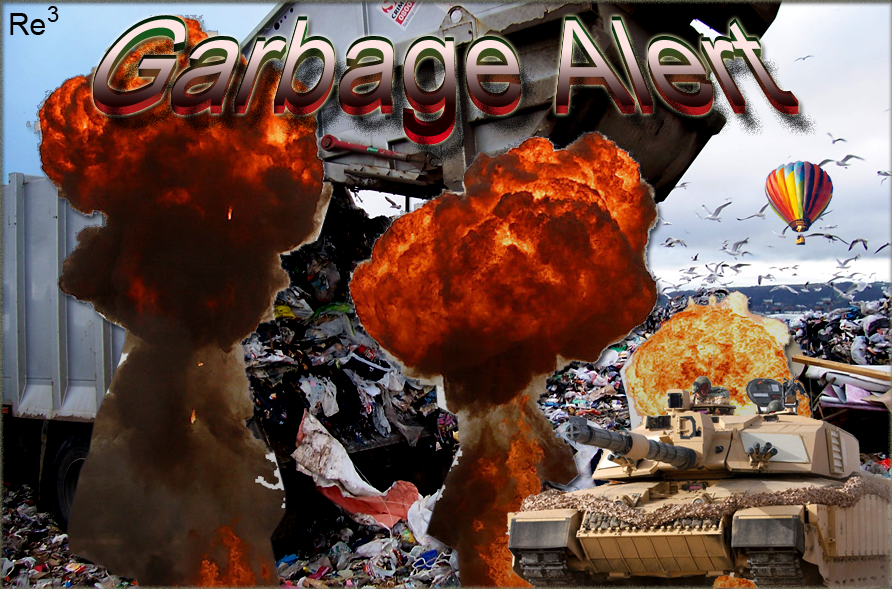
\includegraphics[scale=0.5]{images/splashscreen}
		\end{center}
		\caption{\emph{Garbage Alert} splash screen}
	\end{figure}


Man starter på en øy fylt til randen med søppel. Målet med spillet er å bli
kvitt søppelet. Ved å gjenvinne avfallet får man ulike muligheter til å
bombardere de andre spillerne, forsvare sin egen øy, for så å stå igjen
som vinneren på en øy uten søppel, eller som eneste spiller i live.

Spillet er utviklet av en gruppe studenter på NTNU i faget Eksperter i Team. Spilldesignerne og -utviklerne går under navnet Re³. Re³ består av Andreas Røysland Aarnes, Trond Kjetil Bremnes, Christian Aleksander Lysne, Kjetil Mehl og Ina Sander Pedersen.

Målet med denne seksjonen er å gi deg et innblikk i det utviklede
spillkonseptet, hvilke spillaspekter som er tatt med og spillets
dynamikk.


\subsection{Sjanger}\label{sec:genre}

Et dataspillsjanger er i følge Thomas H. Apperley \cite{sjanger} basert på metodikken og utfordringene i spillet. I motsetning til sjangrer innen litteratur og film er spillsjangrer uavhengig av spillets verden, tidsepoke, visualitet og historie. Det betyr at et spill om en galaktisk krig i fremtiden og et spill om 2. verdenskrig begge er klassifisert som krigsspill. Det er med andre ord utfordringene som må overkommes i spillet som definerer spillets sjanger.
En rekke sjangre ble vurderet for realiseringen av \emph{Garbage Alert}, og disse vil bli beskrevet i korte trekk. Legg dog merke til at navnet ble til en tid etter at sjangeren var valgt.

\subsubsection{Eventyr}
Den første sjangeren som ble vurdert som utgangspunkt for realisering av
spillet var eventyrsjangeren. Denne sjangeren er definert ved at en
direkte kontrollerer en protagonist i en interaktiv historie.
Spilldynamikken består gjerne av det å overvinne ens omgivelser ved
utforskning og oppgaveløsning. Dette er videre forklart i ``Fundamentals
of Game Design''~\cite{game_design}.

Der finnes en hel rekke undersjangrer under eventyrsjangeren. Pek-og-klikk- og action-eventyrsjangrene har vært av spesiell interesse. 

\begin{description}

	\item[Pek-og-klikk-eventyr] \hfill \\

	Her vil en styre protagonisten ved å peke hvor en vil gå, peke på objekter en vil interagere med og peke på andre mennesker en vil snakke med. Underveis samler en objekter som kan brukes andre steder i spillverdenen, enten direkte eller gjennom å kombinere gjenstander med hverandre for å skape nye gjenstander som gjør en i stand til å avansere i spillet.

	Populære spill i denne sjangeren er \emph{Lucas Arts'} \emph{Monkey Island}-serien og \emph{Funcoms} \emph{Den Lengste Reisen}.

	\item[Action adventure] \hfill \\

	Her styrer en tradisjonelt én figur som gradvis finner og samler utstyr som gjør en sterkere og mer motstandsdyktig mot miljø og fiender.


	Populære spill i denne sjangeren er \emph{Nintendos} \emph{The Legend of Zelda} og \emph{Supergiant Games'} \emph{Bastion}.

\end{description}

% \subsection{Rollespill}\label{sec:rollespill}
% RPG



\subsubsection{Strategi}
Den andre sjangeren som ble vurdert for å realisere ideen om et resirkulering- og gjenbruksspill var strategisjangeren. Sentralt i denne sjangeren er ressursforvaltning, noe som også kunne brukes for å realisere et godt konsept.

\begin{description}

	\item[Turbasert strategi] \hfill \\
	Her deles hvert spill inn i \emph{runder}, hvor hver spiller har en egen \emph{tur} til å utføre sine handlinger.


	Den observante leser vil kunne legge merke til at dette ikke er ulikt tradisjonelle brettspill, noe som tilkjennegis ved at mange av de første digitale strategispill var konverteringer av tradisjonelle brettspill.

	Av populære turbaserte strategispill finnes \emph{Firaxis'} \emph{Sid Meier's Civilization} og \emph{Intelligent Systems'} \emph{Advance Wars}. % TODO: Kilder?


	\item[Sanntidsstrategi] \hfill \\
	
I motsetning til turbaserte strategispill vil ikke hver spiller ha sin egen tur til å utføre sine handlinger, men alle spillere vil utføre sine handlinger samtidig.

Blant de mer sentrale elementer ved sanntidsstrategispill er konseptene om ressurshåndtering. De fleste spill i denne sjangeren lar det være opp til brukeren å passe på at man til enhver tid har adekvate ressurser til å gjøre den en ønsker og å benytte seg av de rasjonelt. Et annet element som ofte er til stede er stein-saks-papir-balansering av enheter, hvor enhet A kontrer enhet B, B kontrer enhet C og enhet C kontrer enhet A.

	Av populære sanntidsstrategispill finnes \emph{StarCraft} og \emph{Command \& Conquer}.

\end{description}

\subsubsection{Vårt valg}
Helt i starten av prosessen som førte til \emph{Garbage Alert}, begynte diskusjonen rundt ulike typer eventyr-tilnærminger. Det kan føles svært naturlig, i et spill som skal omhandle resirkulering og gjenbruk, å låne elementer fra den sjangeren som oftest benytter slike mekanismer. Enkelte gruppemedlemmer ønsket dog en mer fartsfull opplevelse, og diskusjoner om å implementere Zelda-aktige elementer i spillet ble tatt opp.

Samtidig ble en alternativ idé utforsket, i kraft av at enkelte ønsket å inkorporere flerspiller og konkurranse som en motivasjonsfaktor. Her startet ideen med å skape et brettspill-inspirert spill. Denne ideen utviklet seg fra å være et svært komplisert turbasert spill, til å bli stadig enklere og raskere, for til slutt å bli et sanntidsstrategispill.

% This is a section where the definition of the game play is established.
% Definitions should include how a player wins, loses, passes levels and
% the main focus of the game play.
\subsection{Definisjoner}
Dette avsnittet forklare de grunnleggende definisjonene rundt Garbage
Alert. Definisjonene er i hovedsak sentrert rundt hvordan spilleren
oppfatter spillet~\cite{gameplay}.
\subsubsection{Oppstart}
Alle spillere starter med like forutsetninger. Hvordan spillet utvikler
seg kommer an på hvordan spillerene bruke ressursene som er gitt.
\subsubsection{Vinning}
En spiller har vunnet dersom alle de andre spillerene har mistet
gjenvinningsstasjonene sine, eller spilleren klarer å blit kvitt alt
søppelet på sin øy.
\subsubsection{Taping}
En spiller taper dersom gjenvinningsstajonen dens blir ødelagt. Spilleren
vil også tape dersom en annen spiller klarer å renske sin øy for søppel.


% List all the elements that are directly related to or to the benefit
% of the player.

% Devise two sets of names for player elements. One set is a generic name
% (or code) and the other is its game name. 

% Describe the terminology that you use to describe the player’s
% properties.

%bruk ord: MILJØSTASJON, GJENVINNING. (ikke gjenvinningstasjon, utvinne, resirkulering)

\subsection{Elementer}
Dette avsnittet forteller om de forskjellige spillelementene som finnes
i Garbage Alert.
\subsubsection{Ressurser}
Ressurser er et viktig element i Garbage Alert. Ressursene er det som
gjør at spillere kan utvikle basen sin, bygge forsvar og utvikle angrep.
Valget av ressurser er basert på Mohs hardhetsskala av mineraler \cite{mohs}. Mohs hardhetskala er en liste over mineraler i rekkefølge etter absolutt hardhet, laget av geologen Friedrich Mohs. Hvert mineral skal kunne skrape mineralet som står foran på listen. Ressursene i Garbage Alert er ikke helt korrekte i forhold til Mohs hardhetsskala, men basert på denne. Idèen er at hver de seks ressursene i spillet følger samme regel, nemlig at den ene ressursen er hardere enn den andre og har mulighet til å ødelegge den. 
De forskjellige typene utvinnbare ressurser er:
\begin{description}
	\item \textbf{Papp}\\ Denne ressursen kan utvinnest uten å måtte
oppgradere miljøstasjonen. Dette er den enkleste ressursen å få fatt i,
men skaper kun relativt svake angrep/forsvar.
	\item \textbf{Plast}\\ Denne ressursen kan man utvinne etter å ha
oppgradert hovedbasen èn gang.
	\item \textbf{Tre}\\ Tre kan utvinnest dersom hovedbasen har blitt
oppgradert til dette. Tre er på samme oppgraderingsnivå som plast, med andre ord må
spilleren velge mellom desse to i begynnelsen. Tre er derimot hardere enn plast i dette spillet.
	\item \textbf{Jern}\\ Jern er mulig å utvinne dersom spilleren først
oppgraderer til tre.
	\item \textbf{Stål}\\ Stål bygger på at spilleren først har
oppgradert til plast.
	\item \textbf{Titan}\\ Titan er den siste ressursen som er mulig å
utvinne. For å kunne utvinne titan må spilleren først ha skaffet seg
alle utvinningsutvidelsene til hovedbasen.
\end{description}


Det er også mulig å skade forsvar/våpen som er bygget av en bedre ressurs enn våpenet. Dette er implementert slik at ingen våpen/forsvar blir uovervinnelige. Figur \ref{fig:ressursoppgraderinger} framstiller hvilke utvidelser man må ha for å kunne oppgradere til neste nivå. Allerede helt fra starten av spillet må man velge om man først vil oppgradere til tre, eller til plast (se seksjon \ref{miljostasjon}). 

	\begin{figure} [H]
				\begin{center}
					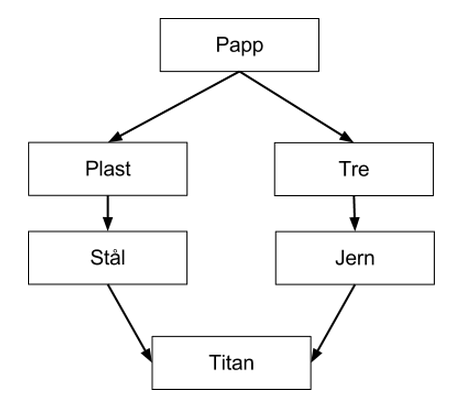
\includegraphics[scale=0.5]{images/oppgraderingstre}
				\end{center}
			\caption{Ressursoppgraderinger}
			\label{fig:ressursoppgraderinger}
	\end{figure}

\subsubsection{Ressursutvinning}
En spiller skaffer seg ressurser ved å gjenvinne søppel som ligger
spredt rundt på øya. Dette blir gjort ved hjelp av miljøstasjonen
som hver spiller starter med.
\subsubsection{Miljøstasjon} \label{miljostasjon}
Miljøstasjonen er det mest sentrale spillelementet i Garbage
Alert. Denne kan bli sett på som hovedbasen i spillet.
Miljøstasjonen kan oppgraderes på tre måter for å forbedre effektiviteten:\\
\begin{description}
	\item \textbf{Volum/Utvinningsgrad}\\Denne oppgraderingen kan øke utvinningsgraden og volumet av søppel som blir brukt i gjennvinningsprosessen. Restavfallet (søppelet som ikke blir gjenvunnet) vil på magisk vis bli borte. Tabell \ref{tab:effektivitet} viser oppgraderingene for Volum/Utvinningsgrad. Man starter på nivå 0, og deretter kan man oppgradere ett trinn ad gangen.
	\item \textbf{Buffer}\\Miljøstasjonen kan få en buffer hvor spilleren kan samle opp søppel, som automatiserer gjenvinningsprosessen til en viss grad. Dermed kan spilleren bruke mindre tid på å sørge for at søppelet på øyen blir flyttet til miljøstasjonen.
	\item \textbf{Ressurser}\\For å kunne gjenvinne nye typer ressurser må
		spilleren oppgradere gjenvinningsstasjonen. Her får spilleren valget
		mellom to ulike veier som vil avgjøre hvilke ressurser spilleren får
		tilgang til (se figur \ref{fig:ressursoppgraderinger}).
\end{description}

\begin{table} \label{tab:effektivitet}
\begin{tabular}[\textwidth]{ l  l  p{3cm}  l  p{4cm} } %\label{tab:effektivitet}
\hline
\bf{Effektivitet} & \bf{Utvinningsgrad} & \bf{Volum} & \bf{Tid} & \bf{Ressurskrav} \\
\hline
Nivå 0 & 10 & 10 & 15sek & Ingen  \\
Nivå 1 & 20 & 10 & 15sek & Papp \\
Nivå 2 & 30 & 10 & 15sek & Papp, og plast eller tre \\
Nivå 3 & 30 & 20 & 15sek & Papp, plast, tre, stål, jern og titan \\
\hline
\end{tabular}
\caption{Oppgraderinger for Volum/Utvinningsgrad}
\end{table}




\subsubsection{Forsvar}
Spillere kan bygge forsvar rundt øya si. Dette forsvaret vil forhindre
motspillere å angripe gjenvinningsstasjonen. Det vil finnes ulike typer
forsvarsmurer, som er kraftige/svake mot ulike typer angrep.
\subsubsection{Angrep}
En spiller får utdelt tre angrepsplattformer. På desse tre platformene
kan spilleren velge hvilke angrep han vil utvikle, basert på hvilke
tilgjengelige ressurser han har.
\subsubsection{Oppgraderinger}
Spilleren har mulighet til å oppgradere både gjenvinningsstasjonen,
våpen og forsvar. Hver type våpen og forsvar har tre nivå, der øking i
nivå vil gi hhv. kraftigere angrep og sterkere forsvar. De tre
våpenplassene på øya kan ha inneholde ulike våpen som kan oppgraderes
hver for seg.
Eksempel på forsvarsoppgradering:\\
Tremur (nivå 1) -> Tremur (nivå 2) -> Tremur (nivå 3).
\begin{quote}
Bør restruktureres!!\\
Spilleren kan utvinne ressurser ved å "dra" søppelenheter fra
forskjellige plasser på øya inn til gjennvinningsstasjonen. Hvilke
ressurser, og mengden av hver ressurs, som spilleren får ut fra en
enkelt søppelenhet er avhengig av nivået på gjennvinningsstasjonen og
hvilke typer oppgraderinger som er gjort. Spilleren kan også bruke sine
våpen til å bli kvitt søppelenheter. Her vil ubehandlede søppelenheter
kunne skytes på motstandere. Effekten av angrepet avhenger av spillerens
våpen, oppgraderingsnivå på våpenet og motstanderens forsvar. For å
beskytte seg mot angrep kan spilleren bygge mur rundt sin øy. Hvilke
våpen og forsvarsmurer som spilleren kan bygge er avhengig av hvilke
ressurser gjenvinningsstasjonen er i stand til å utvinne. Dette betyr at
valg av typer oppgradering for gjenvinningsstasjonen vil være avgjørende
for utviklingen av spillet.\\
\end{quote}

\subsection{Spilldynamikken}
\emph{Garbage Alert} er i utgangspunktet et flerspiller sanntidsstrategispill,
men det er også mulighet for å spille alene mot spillere med kunstig
intelligens. Hver spiller starter med en øy og følgende elementer:
\begin{itemize}
	\item En miljøstasjon
	\item Tre angrepsplattformer
	\item En forsvarssone
	\item 10 enheter med papp i inventaret
	\item 1000 enheter med søppel
	\item Muligheten til å gjenvinne papp fra søppelet. Gjenvinningsgraden er 10\%
	\item Muligheten til å bruke papp til å bygge våpen og forsvar, i form av papirfly og pappmur
	\item Muligheten til å oppgradere gjenvinningsgraden til 20\%
	\item Muligheter for oppgraderinger av gjenvinningsstasjon slik at man også får gjenvunnet plast eller tre.
\end{itemize}

Jo flere typer ressurser man får gjenvunnet fra søppelet, jo flere muligheter har man for mer avanserte våpen, forsvar og oppgraderinger (se seksjon \ref{sec:spillelement}).

%De sentrale spillelementene består av å samle inn søppel til resikulerings vil være samling, %ressursforvaltning, valg av våpen og forsvar, samt timing av våpenbruk. Spillinnholdet vil hovedsaklig være Pure Play (Usikker på dette innebærer det jeg tror), der målet er å få spilleren til å ha det gøy, men det vil også være elementer av realisme da det spilleren foretar seg vil virke inn på både lokalt og globalt miljø. Det vil være en lineær spillsekvens (Er usikker på denne fordi jeg ikke finner noen  spillsekvenstype som passer??) der spilleren får tilgang til nye våpentyper og forsvarsmuligheter etterhvert som krav for hver enkelt oppgradering er nådd. For at spillet skal få et lekent og fristende utseende har vi valgt en type tegneseriestil som vil gjøre nettopp dette. (Husker ikke om vi har vi diskutert dette, og hva vi kom fram til?)\\

%Spillbeskrivelse: Spillets sjanger er valgt til flerspiller sanntidsstrategi, men det vil også være mulighet for å spille alene mot computer. (Usikker på om vi ble enig om at dette skulle være mulig?) Viktige spillelementer vil være samling, ressursforvaltning, valg av våpen og forsvar, samt timing av våpenbruk. Spillinnholdet vil hovedsaklig være Pure Play (Usikker på dette innebærer det jeg tror), der målet er å få spilleren til å ha det gøy, men det vil også være elementer av realisme da det spilleren foretar seg vil virke inn på både lokalt og globalt miljø. Det vil være en lineær spillsekvens (Er usikker på denne fordi jeg ikke finner noen  spillsekvenstype som passer??) der spilleren får tilgang til nye våpentyper og forsvarsmuligheter etterhvert som krav for hver enkelt oppgradering er nådd. For at spillet skal få et lekent og fristende utseende har vi valgt en type tegneseriestil som vil gjøre nettopp dette. (Husker ikke om vi har vi diskutert dette, og hva vi kom fram til?)\\ 

\subsection{Globale og lokale katastrofer}\label{sec:hazards}

I den virkerlige verden har søppel innvirkning på det lokale og globale miljøet. Slik er det også i \emph{Garbage Alert} – jo mer søppel som blir kastet frem og tilbake mellom spillerne, jo høyere blir risikoen for at en katastrofe inntreffer. Spillere som har brukt våpnene mye vil ha en høy risiko for å bli rammet av en lokal katastrofe. Dette gjør at spillet har en høyere vanskeligehetsgrad for de spillerne som ligger godt an sett i forhold til motspillerne. Denne formen for dynamisk vanskelighetsbalansering gjør det slik at en kan hente seg inn igjen selv om en kanskje gjør det litt dårlig i starten.

Den totale våpenkraften som har blitt brukt av alle spillerne er med på å øke sannsynligheten for globale katastrofer. Hver spiller vil ha to måleinstrument på panelet sitt på skjermen som viser sannsynligheten for at en geologisk eller en biologisk katastrofe kan inntreffe, såkalte geohasarder og biohasarder.


\subsubsection{Geohasarder}
Geologiske katastrofer kan intreffe som et resultat av global oppvarming og mekanisk påvirkning fra mennesker.
Et eksempel på en global geologisk katastrofe som kan inntreffe er tsunamier. En tsunami vil gjøre skade på den eventuelle muren spilleren har og muligens også ødelegge våpen og miljøstasjon utover dette. Hvorvidt dette skjer vil bero på murens styrke, som i sin tur beror på murens byggemateriale, og resterende helsepoeng. Eksempler på lokale geologiske katastrofer er jordskjelv og kolliderende isfjell. Jordskjelv gjør en liten skade på alle bygninger på øyen, og et isfjell som kolliderer med øya vil gjøre skade på muren, og muligens ødelegge den avhengig av murens styrke. 

% Si noe om at disse elementene ikke er ferdige?

\subsubsection{Biohasarder}
Et resultat av mye forsøpling av øyene og det omringende havet kan være biologiske katastrofer.
Et eksempel på en global katastrofe som vil ramme samtlige spillere er sur nedbør. Dette vil gi korrosjon av våpen og forsvarsmurer laget av metall og dermed skade disse, samt at planter og trær også vil ta skade og gi øya et trist utseende.

Eksempler på lokale biologiske katastrofer som kan inntreffe er utbrudd av sykdommer på grunn av bakterievekst, som i sin tur gjør at gjenvinning av ressurser på miljøstasjonen og muligheten for våpenangrep stanser opp for en periode.


\subsection{Spillatmosfære}

Ved spillstart er himmelen fylt av mørke skyer og musikken vil ha et melankolsk preg. Stemningen er tung og dyster. Fargene på spillområdet er uklare og skitne fordi øya er forurenset av søppel.
Når søppel fjernes fra øya vil stemningen bli lysere ved at skyene blir hvite og forsvinner med tiden. Musikken blir lystigere, sola kommer fram og fargene på øya øker gradvis i intensitet. Det vil begynne å gro gress, blomster og 
trær på områder av øya som blir frigjort for søppel. Mennesker trives bedre på øya, og små hus vil dukke opp ettersom øya blir renere. 

Stemningen på en ren og fin øy vil forverres dersom den mottar mye søppel fra motstanderne, og det ikke fjernes i tilstrekkelig hastighet,
eller hvis miljøstasjonen på øya ødelegges slik at søppel ikke blir gjenvunnet.
Blomster og trær vil visne når områdene de gror på forurenses av søppel, en klar blå himmel blir dekket av skyer som etterhvert mørkner og
musikken blir jevnt mer melankolsk. 
Når en øy er helt overfylt med søppel vil den synke ned i havet. Dette gjør at havet får et forurenset utseende, og de resterende spillerne vil bli utsatt for en global katastrofe. % Dette nevnes for første gang her.


\subsection{Gameplay og taktikker}

Dette avsnittet vil ta for seg et typisk spill, spilt av tre deltakere som alle bruker forskjellige taktikker. De forskjellige taktikkene er basert på alfa-testing utført av Re³. Hver taktikk vil få en kort beskrivelse hvor fordeler og ulemper vil bli nevnt. Antall ressurser og helsepoeng vil ikke gis i detalj.

De tre deltakerne i spillet er: \emph{Professor}; \emph{MadMax}; og \emph{N00b87}. Spillet starter og hver spiller ser på en mørk øy fylt til randen av søppel. Det er en dyster og melankolsk stemning, og man får en følelse av at man har reist fram i tid til et post-apokalyptisk samfunn.

Spilleren med navnet Professor har valgt å kun fokusere på oppgraderinger knyttet til effektivitet for å raskt bli kvitt søppelet sitt gjennom gjenvinning på miljøstasjonen. Denne taktikken kan raskt avslutte spillet, men risikoen er meget høy. Dersom Professor blir angrepet må han endre taktikk raskt. Forhåpentligvis kommer ikke angrepene med en gang, og han vil raskt ha flere ressurser enn de andre spillerne. Etterhvert som spillet går bør Professor bygge en mur, for å unngå at et enkelt angrep med et høyt utviklet våpen tar miljøstasjonen hans på ett skudd. Dersom han klarer å komme seg til effektivitetsnivå 3 før han blir angrepet, blir han veldig raskt kvitt søppelet sitt, ettersom denne oppgraderingen dobler gjenvinningsraten. 

Spilleren MadMax velger å kjøre en aggresiv taktikk. Det første han gjør er å bygge et papirfly, slik at han allerede fra starten klarer å dumpe noe av søppelet sitt på de andre spillerne. Fordelen med et kjapt angrep er at spillerne som blir angrepet alltid vil ligge et skritt bak, og ikke kunne angripe han tilbake. Det første de andre spillerne vil gjøre etter et angrep er å sikre miljøstasjonen sin mot utslettelse ved å bygge en mur. MadMax kan dermed bruke ressursene sine på våpen hele tiden, mens de andre spillerne må fortsette å reparere og bygge muren sin. MadMax er avhengig av å utslette de andre spillerne eller sende bort alt søppelet sitt raskt. Hvis det tar for lang tid vil de andre spillerne etterhvert få bedre oppgraderinger, og MadMax sine angrep vil til slutt ikke kunne penetrere muren til de andre spillerne.

Den tredje spilleren, N00b87, bestemmer seg for en defensiv og sikker spilltaktikk. Spilleren satser på å komme seg raskt gjennom oppgraderingene, samtidig som han hele tiden oppgraderer muren og våpnene sine. Ettersom N00b87 bruker ressurser på alt som er tilgjengelig bruker han lengre tid på å utvikle seg enn de andre spillerne. Men N00b87 er likevel godt sikret mot angrep, og kan raskt gjøre et motangrep som forhåpentligvis roer aggresiviteten til eventuelle angripere. Denne taktikken har få overaskelsesmomenter, men likevel anses dette som taktikken som oftest vil vinne. Men det er også mange momenter som fører til at denne ``sikre'' taktikken ikke vil vinne. Ettersom N00b87 ikke angriper så har Professor mulighet til å bli kvitt alt sitt søppel lenge før N00b87. Dersom MadMax angriper N00b87 helt fra starten, vil N00b87 slite med å komme seg gjennom planen sin. 

Det er ingen taktikk som er best. Det er mange tilfeldigheter som kan snu spillet. Hvem blir angrepet? Blir en spiller angrepet av mange spillere er spilleren dømt fra starten. Globale og lokale katastrofer vil også bidra til å snu spillet, og kan til og med overraske den klare lederen av et spill. Det er tre spillere i eksempelet over, og det er helt åpent hvem som kan vinne!

Adrenalinet av å bombe de andre spillerne og å selv bli knust; raske avgjørelser for å kjapt hente seg inn eller ta nådestøtet for å ta seieren; valg av taktikker som kan overraske de andre spillerne; plutselige katastrofer som kan snu spillet mot alle retninger. Denne spenningen er noe av det som gjør \emph{Garbage Alert} til et kjekt spill som til og med får din bestemor til å trekke på smilebåndet.

% This is a spreadsheet containing the generic names of the player and
% antagonistic elements and their game properties. 

% This should allow an easy cross reference for an elements in the game
% that a value. 
\subsection{Spillmatrisen}
Spillmatrisen (se figur \ref{fig:spillmatrise}) er en grafisk forklaring
på hvilke elementer i spillet som interagerer med hverandre. Elementer
som våpen, forsvar og oppgraderinger er kun beskrevet på et overordnet
nivå, siden disse elementene deler like egenskaper (for eksempel at alle
angrep kan angripe forsvar).
\begin{center}
\begin{figure} [H]
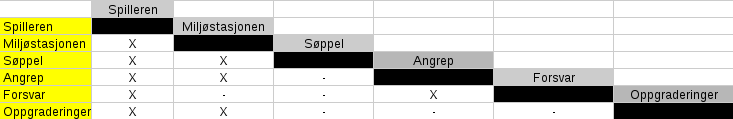
\includegraphics[scale=0.6]{images/spillmatrise.png}
\caption{Spillmatrise med de forskjellige elementene}
\label{fig:spillmatrise}
\end{figure}
\end{center}
I figur~\ref{fig:spillmatrise} er elementene som interagerer merket
med en \textbf{X} i den kolonnen og raden elementene sammenfaller.
Hvordan elementene interagerer er beskrevet nedenfor:
\begin{description}
\item \textbf{Spilleren}\\Spilleren sin oppgave er å samle søppel,
bygge våpen og forsvar, samt oppgradere miljøstasjonen.
\item \textbf{Miljøstasjonen}\\Miljøstasjonen tar imot og gjenvinner
søppelet. I tillegg er dette hovedbasen for spilleren, og står for alle
oppgraderingene. En miljøstasjon kan bli angrepet av andre spillere, og
interagerer derfor med våpen.
\item \textbf{Søppel}\\Søppel blir plukket opp av spilleren, og lagt på
miljøstasjonen for gjenvinning.
\item \textbf{Angrep}\\Spillere kan angripe andre spillere sitt forsvar, angrep (våpen) 
og miljøstasjonene deres.
\item \textbf{Forsvar}\\Forsvaret kan bli angrepet og ødelagt av våpen.
En spiller bygger forsvaret, og har derfor interaksjonen mellom spiller og forsvar.
\item \textbf{Oppgraderinger}\\Spilleren kan oppgradere miljøstasjonen
sin. Disse oppgraderingene baserer seg på statusen til miljøstasjonen.
\end{description}
% Make a list of all objects that affect the player in a positive way.
% (i.e. health replenished)

% Define these objects by describing what affect they cause and how the
% player can use the object.
\subsection{Spillkonsekvenser}
Dette delkapittelet forteller om de forskjellige negative og positive
konsekvensene en spiller kan og vil oppleve gjennom spillets gang. Disse konsekvensene har som hensikt å underbygge landsbyens overordnede tema, som et ledd i å hjelpe spilleren til å forstå hva en gjør som er riktig, og hva en gjør som er galt.

Gjennom å oppgradere miljøstasjonen og dermed kunne bedre håndtere søppelet på øya vil en kunne visuelt se at øya blir renere, atmosfæren blir klarere og bakgrunnsmusikken blir penere. Lystige lydeffekter signaliserer at en gjør noe som gir spilleren en fordel i forhold til motspillerne, for eksempel når spilleren oppgraderer utstyr eller utfører et vellykket angrep mot sine
motstandere. Dette skal skaper en positiv mestringsfølelse hos spilleren. 

Videre er der en intrisitt verdi i å vinne et spill over ens
medspillere.

For å kunne underbygge spillets underliggende tematikk om
miljøvennlighet vil naturen straffe spillerne som ikke tenker miljø.
Geologiske og biologiske katastrofer er konsekvensene som rammer en
eller alle spillerne.
På samme måte som at muntre lydeffekter underbygger gode handlinger
gjort av spilleren, vil dystre lydeffekter signalisere negative
hendelser. Dette kan for eksempel være i det en blir angrepet av
motspillerne. 

Når en vinner eller taper et spill vil dette føres opp på spillerens
profil. Med dette kan hver spiller ha oversikt over sin egen
spillstatistikk. På spillerens profil finnes det også et profilbilde av
en kriger. Bildet vil også være synlig for de spillerne man spiller mot
under et spill. Man begynner med et standard profilbilde, og etterhvert
som man vinner mange spill får man muligheten til å endre dette bilde.
Målet med dette er å gi spilleren en visuell prestasjonspremie, i
tillegg får de spillerne man spiller mot en idé om hvor mye motspilleren
har spilt spillet tidligere.
% This is where a description of the user’s control of the game can be
%placed.

% It is also recommended to think about which buttons on a device would
% be best suited for the game.

% Consider what the worst layout is, then ask you self if your UI is it
% still playable?

% A visual representation can be added, where we relate the physical
% controls to the actions in the game.


% TODO
% * Skrive om de svakeste elementene i grensesnittet
% * Referere til screenshots
% * Inkludere noe tekst om lydbildet?
% * Generell formattering, sammenslåing og sortering av avsnitt

\subsection{Brukergrensesnitt}

Brukergrensessnittet i spillprototypen er svært uferdig, men noe av funksjonaliteten er på plass for å bedre kunne illustrere våre ideer og tanker rundt konseptet. 
For å gjøre spillet tilgjengelig for vår målgruppe er \emph{Garbage Alerts} brukergrensesnitt på norsk, samt at spillets figurer og illustrasjoner er ment å være stiliserte og enkle å forstå.


Det man først ser når man starter spillet er en introskjerm som med sin overdrevne grafikk og lydbilde er ment å sette spilleren i et kompetetivt sinnelag.
Fra denne skjermen er det mulig å starte spillet ved å trykke på den store knappen markert ``Start''.
En komplett versjon av spillet vil gi spilleren flere valg på introskjermen, som å endre spillernavn, samt gi muligheten til å koble flere spillere sammen i et flerspillerspill.


Spillets hovedskjerm\footnote{Den delen av spillet hvor spillet faktisk spilles.} består av et overblikksbilde av alle øyene som er med i spillet. I prototypen er antallet begrenset til to, men en mer moden versjon vil inneholde muligheten til å spille flere enn to stykker samtidig. En skiller mellom seg selv og andre ved bruk av ulike farger på spillernes miljøstasjon, våpen og forsvar. I prototypen er de to faksjonene farget rød og blå.

I prototypen er hovedskjermen et statisk fugleperspektiv av alle øyene og alle spillets elementer. En ferdig versjon vil også inneholde muligheten til å veksle mellom et detaljbilde av spillerens egen øy og et overblikksbilde over alle øyer. Hvorvidt dette vil gjøres via en knapp som veksler mellom de to visningsmodi eller om en vil ``klype for å zoome'' er på dette stadiet noe uvisst og bør testes via brukertesting for å finne den optimale metoden.

\emph{Garbage Alert} er tenkt å først og fremst spilles på mobiltelefoner og andre enheter med berøringsskjerm. Man interagerer derfor med elementene på skjermen ved å trykke på de. Det man må være spesielt oppmerksom på med slike skjermer er å holde knapper store nok, samt at alle elementer på skjermen må være forskjellige nok til at det er enkelt å skille dem fra hverandre på små skjermer.

Spillet kan også spilles på en datamaskin i en nettleser, og en kan derfor også bruke en musepeker for å trykke på elementene på samme måte.

Merk at det under utviklingen kun er testet en prototype på en dataskjerm, og spillet er per nå ikke  tilpasset mobiltelefoner i like stor grad som det burde være. Enkle tester på mobiltelefon har dog blitt utført, men har vært nedprioritert grunnet tidspress.
